%% LyX 2.3.6.1 created this file.  For more info, see http://www.lyx.org/.
%% Do not edit unless you really know what you are doing.
\documentclass[english]{article}
\usepackage[T1]{fontenc}
\usepackage[latin9]{inputenc}
\usepackage{geometry}
\geometry{verbose,tmargin=2.5cm,bmargin=2.5cm,lmargin=2.5cm,rmargin=2.5cm}
\usepackage{color}
\usepackage{array}
\usepackage{multirow}
\usepackage{amsmath}
\usepackage{graphicx}
\PassOptionsToPackage{normalem}{ulem}
\usepackage{ulem}

\makeatletter

%%%%%%%%%%%%%%%%%%%%%%%%%%%%%% LyX specific LaTeX commands.
%% Because html converters don't know tabularnewline
\providecommand{\tabularnewline}{\\}

\makeatother

\usepackage{babel}
\begin{document}
{[}SPLIT\_HERE{]}
\begin{enumerate}
\item \textbf{{[}NYJC/PRELIM/9569/2020/P2/Q1{]} }

The task is to implement a hash table to retrieve data about waste
disposal in Singapore. 

For each of the sub-tasks, add a comment statement, at the beginning
of the code using the hash symbol '\texttt{\#}', to indicate the sub-task
the program code belongs to, for example:
\noindent \begin{center}
\begin{tabular}{c|l|}
\cline{2-2} 
\multirow{2}{*}{\texttt{In{[}1{]}:}} & \texttt{\# Task 1.1}\tabularnewline
 & \texttt{Program Code}\tabularnewline
\cline{2-2} 
\multirow{2}{*}{\texttt{In{[}2{]}:}} & \texttt{\# Task 1.2}\tabularnewline
 & \texttt{Program Code}\tabularnewline
\cline{2-2} 
\multirow{2}{*}{\texttt{In{[}3{]}:}} & \texttt{\# Task 1.3}\tabularnewline
 & \texttt{Program Code}\tabularnewline
\cline{2-2} 
\multicolumn{1}{c}{} & \multicolumn{1}{l}{\texttt{Output:}}\tabularnewline
\end{tabular}
\par\end{center}

The file \texttt{waste.csv} contains the following fields in each
line: 

\texttt{Year \textendash{} \textquotedblleft YYYY\textquotedblright{} }

\texttt{Waste Disposed Of \textendash{} \textquotedblleft Numeric\textquotedblright{}
(Million Tons) }

\texttt{Waste Recycled \textendash{} \textquotedblleft Numeric\textquotedblright{}
(Million Tons) }

The first line of the file contains the headings. 

\subsection*{Task 1.1 }

Write a program to: 
\begin{itemize}
\item read data from \texttt{waste.csv} 
\item into a hash table of size 20 
\item by creating a function \texttt{GetKeyAddress(Year)} to generate the
hash address 
\item and directly inserting the data into the correct location in the hash
table 
\item taking care of any potential collisions using any suitable methods 
\end{itemize}
Display the contents of the hash table showing the data from the first
slot to the last slot. \hfill{}{[}14{]}

\subsection*{Task 1.2}

Create a menu with the following options: 
\begin{enumerate}
\item[1.] \texttt{ Get Waste Disposed and Recycled by year }
\item[2.] \texttt{ Display year(s) where Recycled waste > Waste disposed }
\item[3.] \texttt{ Return Average waste disposed between two years }
\item[4.] \texttt{ -1 to Exit }
\end{enumerate}
\begin{itemize}
\item implement the functions for each menu choice. 
\item use only direct access to retrieve data for options 1 and 3. 
\item option 1 and 3 requires asking users to input in the year(s). 
\item validate the user input. 
\item test option 1 with the year 2007 and show the output. 
\item test option 3 with the range 2002 to 2008 and show the output. 
\item show the output for option 2. \hfill{}{[}10{]}
\end{itemize}
Save your program code and output for Task 1 as 

\texttt{TASK1\_<your name>.ipynb }

{[}SPLIT\_HERE{]}
\item \textbf{{[}NYJC/PRELIM/9569/2020/P2/Q2{]} }

A school library stores the following data in a file named \texttt{story.csv}: 

\begin{tabular}{ll}
\textbf{Field} & \textbf{Format}\tabularnewline
book\_title & text\tabularnewline
text subject & text\tabularnewline
author\_name & text\tabularnewline
published & \textquoteleft YYYY\textquoteright{} (year) \tabularnewline
\end{tabular}

Merge sort is an efficient sorting algorithm which falls under divide
and conquer paradigm and produces a stable sort. It operates by dividing
a large array into two smaller subarrays and then recursively sorting
the subarrays. 

For each of the sub-tasks, add a comment statement at the beginning
of the code using the hash symbol '\texttt{\#}', to indicate the sub-task
the program code belongs to, for example: 
\noindent \begin{center}
\begin{tabular}{c|l|}
\cline{2-2} 
\multirow{2}{*}{\texttt{In{[}1{]}:}} & \texttt{\# Task 2.1}\tabularnewline
 & \texttt{Program Code}\tabularnewline
\cline{2-2} 
\multirow{2}{*}{\texttt{In{[}2{]}:}} & \texttt{\# Task 2.2}\tabularnewline
 & \texttt{Program Code}\tabularnewline
\cline{2-2} 
\end{tabular}
\par\end{center}

\subsection*{Task 2.1 }

Write program code to: 
\begin{itemize}
\item read data from \texttt{story.csv} into an array of records. 
\item ask user to input in which field to sort the records by.
\item validate that the choice must be \texttt{\textquoteleft B\textquoteright },
\texttt{\textquoteleft S\textquoteright }, \texttt{\textquoteleft A\textquoteright },
or \texttt{\textquoteleft P\textquoteright{}} representing \texttt{book\_title},
\texttt{subject}, \texttt{author\_name} and \texttt{published} fields. 
\item implement a \texttt{MergeSort(ArrayData, Sortby)} function that takes
in two parameters, \texttt{ArrayData} (array of records) and \texttt{Sortby},
and sorts the records in ascending order according to the specified
field. \texttt{MergeSort(ArrayData, Sortby)} will return the sorted
\texttt{ArrayData} using a mergesort algorithm to do the sorting. 
\item display \texttt{ArrayData}. 
\item test your program twice and show your output for sorting by \texttt{subject}
and by \texttt{author\_name}. \hfill{} {[}12{]}
\end{itemize}

\subsubsection*{Task 2.2 }

Write program code to: 
\begin{itemize}
\item implement a \texttt{QuickSort(ArrayData)} function that uses the quicksort
algorithm to sort the \texttt{ArrayData} by \texttt{book\_title} in
descending order. \hfill{} {[}8{]}
\end{itemize}
Design 2 test cases to test your QuickSort(ArrayData) function and
explain the purpose of the test data. Show the output of your test
cases. \hfill{}{[}4{]}

Save your program code and output for Task 2 as 

\texttt{TASK2\_<your name>.ipynb}

{[}SPLIT\_HERE{]}
\item \textbf{{[}NYJC/PRELIM/9569/2020/P2/Q3{]} }

You are to create a song playlist using a doubly linked list implemented
using Object-Oriented Programming (OOP). The doubly linked list data
structure is a linked list made up of nodes with two pointers pointing
to the next and previous element. 
\begin{center}
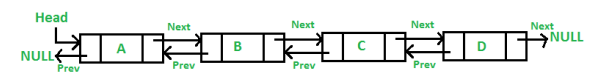
\includegraphics[width=0.5\paperwidth]{C:/Users/Admin/Desktop/Github/question_bank/LyX/static/img/9569-NYJC-2020-P2-Q3-1}
\par\end{center}

A doubly linked list allows traversal of nodes in both direction which
is not possible in a singly linked list. For example, a user can go
forward or backwards to play the next or previous song.

The \texttt{node}, will store the following data: 
\begin{itemize}
\item \texttt{title (str) }
\item \texttt{prev (node) }
\item \texttt{next (node)} 
\end{itemize}
The class, \texttt{SongPlaylist}, will store the following data: 
\begin{itemize}
\item a doubly linked list of \texttt{node} objects. 
\item \texttt{head} pointer, pointing to the first \texttt{node} in the
doubly linked list. 
\end{itemize}
The class \texttt{SongPlaylist} has the following methods: 
\begin{itemize}
\item \texttt{insert(SongPlaylist, title: str)} adds a song title at the
beginning of the list. 
\item \texttt{insertafter(SongPlaylist, searchtitle: str, newtitle: str)}
adds a song title after \texttt{searchtitle}.
\item \texttt{display(SongPlaylist)} outputs out the playlist. 
\end{itemize}
For each of the sub-tasks, add a comment statement, at the beginning
of the code using the hash symbol '\#', to indicate the sub-task the
program code belongs to, for example: 
\noindent \begin{center}
\begin{tabular}{c|l|}
\cline{2-2} 
\multirow{2}{*}{\texttt{In{[}1{]}:}} & \texttt{\# Task 3.1}\tabularnewline
 & \texttt{Program Code}\tabularnewline
\cline{2-2} 
\multirow{2}{*}{\texttt{In{[}2{]}:}} & \texttt{\# Task 3.2}\tabularnewline
 & \texttt{Program Code}\tabularnewline
\cline{2-2} 
\multirow{2}{*}{\texttt{In{[}3{]}:}} & \texttt{\# Task 3.3}\tabularnewline
 & \texttt{Program Code}\tabularnewline
\cline{2-2} 
\multicolumn{1}{c}{} & \multicolumn{1}{l}{\texttt{Output:}}\tabularnewline
\end{tabular}
\par\end{center}

\subsection*{Task 3.1 }

Write program code to define classes to implement the song playlist.
The figures below show the links that must be updated for the insert
and insertafter methods: 

Inserting at the beginning of the list
\begin{center}
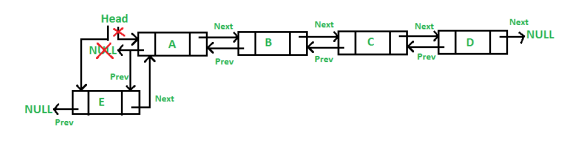
\includegraphics[width=0.5\paperwidth]{C:/Users/Admin/Desktop/Github/question_bank/LyX/static/img/9569-NYJC-2020-P2-Q3-2}
\par\end{center}

Inserting after a given node
\begin{center}
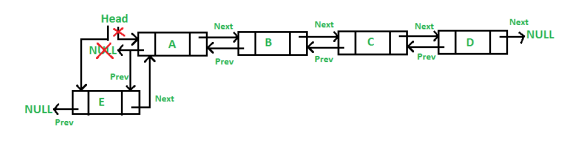
\includegraphics[width=0.5\paperwidth]{C:/Users/Admin/Desktop/Github/question_bank/LyX/static/img/9569-NYJC-2020-P2-Q3-3}
\par\end{center}

\noindent \begin{center}
\textcolor{white}{.}\hfill{}{[}10{]} 
\par\end{center}

The program has the following menu: 
\begin{enumerate}
\item[1.] \texttt{ Create New Song Playlist }
\item[2.] \texttt{ Add a song in front }
\item[3.] \texttt{ Add a song after }
\item[4.] \texttt{ Display Playlist }
\item[5.] \texttt{ -1 to End }
\end{enumerate}
Option 1 will prompt the user to enter the name of the new playlist. 

Option 2 will prompt the user to enter the song title and the name
of the playlist. 

Option 3 will prompt the user to enter the name of the playlist, existing
song title, and the new song title to be inserted after the existing
song title. 

Option 4 will prompt the user to enter the name of the playlist to
be displayed and output accordingly. 

\subsection*{Task 3.2 }

Write program code to: 
\begin{itemize}
\item display the main menu. 
\item input the choice by the user. 
\item run the appropriate code to carry out the task for the choice made.
\hfill{}{[}4{]}
\end{itemize}
Test your program by creating a new playlist called \texttt{MJ} and
add in the following titles in order: \texttt{\textquotedblleft Heal
the World\textquotedblright }, \texttt{\textquotedblleft Thriller\textquotedblright },
\texttt{\textquotedblleft Beat It\textquotedblright }. Show your output
by displaying the playlist.\hfill{}{[}2{]}

\subsection*{Task 3.3 }

Extend your program by writing a function \texttt{insertionSort(Playlist)}
that will sort the song titles in ascending order. 

The algorithm for this \texttt{insertionSort} is given below: 
\begin{enumerate}
\item[1)]  Create an empty \texttt{sorted} doubly linked list. 
\item[2)]  Traverse the given doubly linked list, do following for every node.
- Insert current node in sorted way in \texttt{sorted} doubly linked
list. 
\item[3)]  Change head of given linked list to head of \texttt{sorted} list. 
\end{enumerate}
Write program code to implement \texttt{insertionSort(Playlist)}.
\hfill{}{[}6{]}

Save your program code and output for Task 3 as 

\texttt{TASK3\_<your name>.ipynb} 

{[}SPLIT\_HERE{]}
\item \textbf{{[}NYJC/PRELIM/9569/2020/P2/Q4{]} }

A school wants to create a database to allow students to register
for different enrichment activities that will be held on the school\textquoteright s
Enrichment Day. An enrichment activity falls under one of three categories
-- Arts, Cultural, and Sports. 

It is expected that the database should be normalised. 

When a student registers for an activity, the following information
is recorded: 
\begin{itemize}
\item \texttt{StudentID} - unique 6-digit register number of the student. 
\item \texttt{Type} - type of activity (\texttt{'A\textquoteright }, \texttt{\textquoteleft C\textquoteright{}}
or \texttt{'S'}). 
\item \texttt{Venue} - where the activity will be held. 
\item \texttt{Session} - whether the activity is conducted in the morning
or afternoon (\texttt{'AM'} means the morning session, and \texttt{'PM'}
means the afternoon session). 
\end{itemize}
For the Arts category, the following extra information is recorded: 
\begin{itemize}
\item \texttt{Performance} -- \textquotedblleft \texttt{True}\textquotedblright{}
for performance arts, \textquotedblleft \texttt{False}\textquotedblright{}
for visual arts. 
\end{itemize}
For Cultural, the following extra information is recorded:
\begin{itemize}
\item \texttt{Race} -- which race the culture belongs to. 
\end{itemize}
For Sports, the following extra information is recorded: 
\begin{itemize}
\item \texttt{Contact} -- \textquotedblleft C\textquotedblright{} to denote
contact sports, \textquotedblleft NC\textquotedblright{} to denote
non-contact sports. 
\item \texttt{Cost} - the amount of money in dollars (not more than \$50)
the student must pay the instructor. 
\end{itemize}
The information is to be stored in four different tables: 

\texttt{Registration }

\texttt{Arts}

\texttt{Cultural }

\texttt{Sports }

\subsection*{Task 4.1}

Create an SQL file called\texttt{ TASK4\_l\_<your name>.sql} to show
the SQL code to create the database\texttt{ register.db} with the
four tables. The table, \texttt{Registration}, must use \texttt{StudentID}
as its \textbf{primary key}. The other tables must refer to the \texttt{StudentID}
as a \textbf{foreign key}.

Save your SQL code as 

\texttt{TASK4\_1\_<your name>.sql}\hfill{} {[}5{]}

\subsection*{Task 4.2 }

The school wants to allow students to register over the internet.
The form design for the webpage is shown below: 
\begin{center}
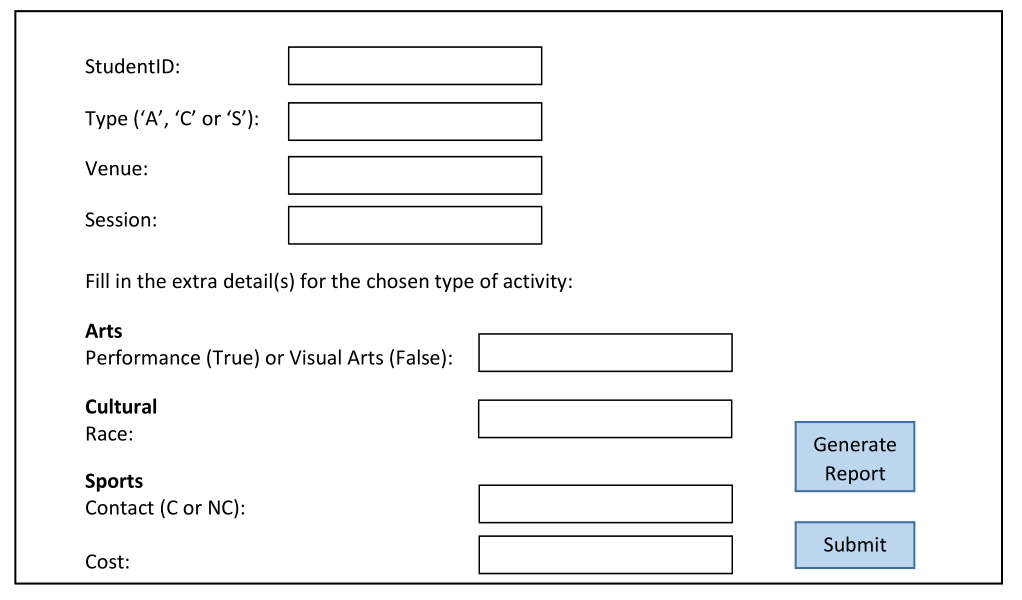
\includegraphics[width=0.5\paperwidth]{C:/Users/Admin/Desktop/Github/question_bank/LyX/static/img/9569-NYJC-2020-P2-Q4}
\par\end{center}

Write a Python program and the necessary files to create a web application
that: 
\begin{itemize}
\item accepts the input from the web form (assume input is keyed in correctly) 
\item updates the registration details into \texttt{register.db} 
\item creates and returns a HTML document that enables the web browser to
display a table tabulating the \texttt{StudentID} and \texttt{Type}
of activity registered for the morning session. 
\end{itemize}
Save your Python program as

\texttt{TASK4\_2\_<your name>.py} with any additional files / sub-folders
as needed in a folder named \texttt{TASK4\_2\_<your name>} \hfill{}{[}12{]}

\subsection*{Task 4.3 }

Test your web application by entering the following records via the
form\textquoteright s submit button: 

\texttt{192701, A, Hall, AM, True }

\texttt{192703, A, MPR, PM, False }

\texttt{192723, S, Field, AM, C, 20 }

\texttt{192803, C, 5-56, AM, Malay }

\texttt{192820, S, 5-60, PM, NC, 15 }

\texttt{193005, C, LT4, PM, Chinese }

\texttt{193006, C, LT4, PM, Chinese} 

Save the output of the program when the user clicks on the \textquotedblleft Generate
Report\textquotedblright{} button as \texttt{TASK4\_3\_<your name>.html}\hfill{}
{[}3{]}

\subsection*{Task 4.4 }

Write SQL code to count the number of different races for the cultural
activities. Run this query. 

Save this code as 

\texttt{TASK4\_4\_<your name>.sql} \hfill{}{[}4{]}

{[}SPLIT\_HERE{]}
\item \textbf{{[}NYJC/PRELIM/9569/2020/P1/Q1{]} }

\textbf{Figure 1} shows ten numbers stored in an array \texttt{L}.
\noindent \begin{center}
\begin{tabular}{|c|c|c|c|c|c|c|c|c|c|}
\multicolumn{10}{c}{\textbf{Figure 1}}\tabularnewline
\hline 
\multicolumn{10}{|c|}{\texttt{L}}\tabularnewline
\hline 
\texttt{{[}1{]}} & \texttt{{[}2{]}} & \texttt{{[}3{]}} & \texttt{{[}4{]}} & \texttt{{[}5{]}} & \texttt{{[}6{]}} & \texttt{{[}7{]}} & \texttt{{[}8{]}} & \texttt{{[}9{]}} & \texttt{{[}10{]}}\tabularnewline
\hline 
\texttt{34} & \texttt{8} & \texttt{6} & \texttt{35} & \texttt{27} & \texttt{35} & \texttt{63} & \texttt{56} & \texttt{16} & \texttt{24}\tabularnewline
\hline 
\end{tabular}
\par\end{center}

The numbers in \texttt{L} are to be sorted.

\textbf{Figure 2} shows an \textbf{incomplete} structure chart that
has been created while developing a solution to the problem of sorting
the numbers in \texttt{L}.

The constant \texttt{MAX} has been used to represent the size of the
array.
\noindent \begin{center}
\textbf{Figure 2} 
\par\end{center}

\begin{center}
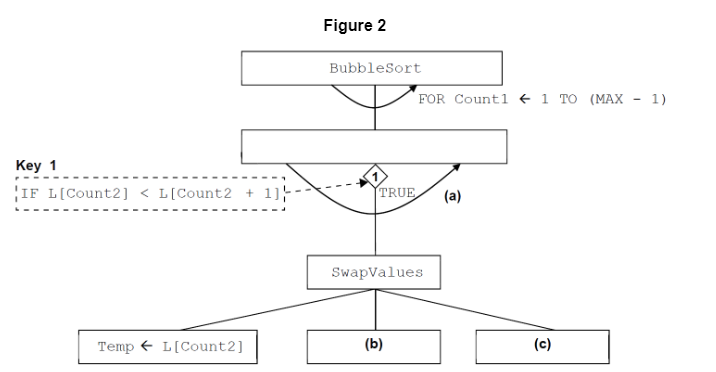
\includegraphics[width=0.5\paperwidth]{C:/Users/Admin/Desktop/Github/question_bank/LyX/static/img/9569-NYJC-2020-P1-Q1}
\par\end{center}
\begin{enumerate}
\item {}
\begin{enumerate}
\item Describe the goal of this problem. \hfill{}{[}1{]}
\item How should the curved arrow \textbf{(a)} in \textbf{Figure 2} be labelled?
\hfill{}{[}1{]}
\item What should be written in box \textbf{(b)} in \textbf{Figure 2}? \hfill{}{[}1{]}
\item What should be written in box\textbf{ (c)} in \textbf{Figure 2}? \hfill{}{[}1{]}
\end{enumerate}
\end{enumerate}
A new Bubble Sort routine is developed using the structure chart shown
in \textbf{Figure 2}.
\begin{enumerate}
\item[(b)] What value will be in \texttt{L{[}1{]} }when this Bubble Sort routine
has finished executing on the array \texttt{L} shown in \textbf{Figure
1}? \hfill{}{[}1{]}
\item[(c)]  A Bubble Sort routine, based on the structure chart in \textbf{Figure
2}, always completes \texttt{MAX - 1} passes through the array. Often,
this number of passes is not required, as the contents of the array
will be sorted after fewer passes have been made. If a pass is made
through the array during which no swaps need to be made, then the
array has been sorted.

Describe the changes that need to be made to the Bubble Sort routine
so that it will only complete the minimum number of passes through
the array that are needed to fully sort the contents of the array.
\hfill{} {[}3{]}
\item[(d)] The Bubble Sort routine can also be implemented using recursion. 
\begin{enumerate}
\item Define what is meant by a recursive function. \hfill{} {[}2{]}
\item Using pseudocode, write a recursive Bubble Sort routine.\hfill{}
{[}3{]}
\item Explain a disadvantage of a recursive Bubble Sort function over an
iterative one.\hfill{} {[}2{]}
\item Name and describe another recursive sort algorithm. \hfill{} {[}5{]}
\end{enumerate}
\end{enumerate}
{[}SPLIT\_HERE{]}
\item \textbf{{[}NYJC/PRELIM/9569/2020/P1/Q2{]} }

In Morse code, each letter of the alphabet is represented by a unique
combination of dots and dashes. Study the following table carefully:
\noindent \begin{center}
\begin{tabular}{|c|c|c|}
\hline 
\textbf{Letter} & \textbf{Morse Code} & \tabularnewline
\hline 
\hline 
A & \texttt{. -} & dot dash\tabularnewline
\hline 
B & \texttt{- . . .} & dash dot dot dot\tabularnewline
\hline 
C & \texttt{- . - .} & dash dot dash dot\tabularnewline
\hline 
D & \texttt{- . . .} & dash dot dot\tabularnewline
\hline 
\end{tabular}
\par\end{center}

A binary tree is used to represent this coding system. Each node,
except the root node, contains a letter of the alphabet. The position
of each letter in the tree is determined by its Morse code. Moving
from one node to another down the tree is done by traversing either
a left branch or a right branch. A left branch corresponds to a .
(dot) and a right branch corresponds to a -- (dash). 

The first three levels of the tree are shown below:
\begin{center}
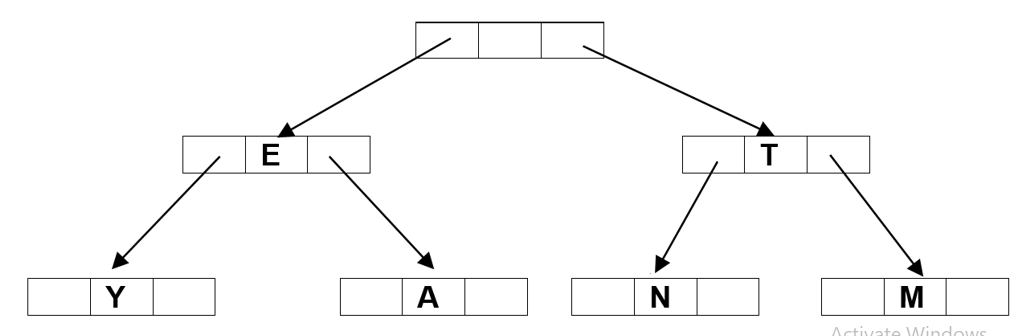
\includegraphics[width=0.5\paperwidth]{C:/Users/Admin/Desktop/Github/question_bank/LyX/static/img/9569-NYJC-2020-P1-Q2}
\par\end{center}
\begin{enumerate}
\item What are the Morse codes for the letters N and Y? \hfill{}{[}2{]}
\item Draw a diagram of the binary tree which clearly shows the position
of the letters D, C and B in the tree.\hfill{} {[}3{]}
\item {}
\begin{enumerate}
\item Explain why this binary tree representation is not the most suitable
data structure for performing English to Morse code conversion. \hfill{}{[}2{]}
\item Describe a better alternative and explain how the Morse code of a
letter could be found. \hfill{}{[}3{]}
\end{enumerate}
\end{enumerate}
{[}SPLIT\_HERE{]}
\item \textbf{{[}NYJC/PRELIM/9569/2020/P1/Q3{]} }

The algorithm represented using pseudo-code in \textbf{Figure 3} describes
a method to convert two hexadecimal numbers into decimal. The subroutine
\texttt{ToDecimal} used in\textbf{ Figure 3} is shown in \textbf{Figure
4} and the built-in subroutine \texttt{ASCII} is explained in \textbf{Table
1}. 
\noindent \begin{center}
\textbf{Figure 3} 
\par\end{center}

\noindent %
\noindent\begin{minipage}[t]{1\columnwidth}%
\texttt{FOR Count <- 1 TO 2 }

\texttt{\qquad{}INPUT HexString }

\texttt{\qquad{}Number <- 0 }

\texttt{\qquad{}FOR EACH HexDigit IN HexString }

\texttt{\qquad{}\qquad{}Value <- ToDecimal(HexDigit) }

\texttt{\qquad{}\qquad{}Number <- Number {*} 16 + Value }

\texttt{\qquad{}ENDFOR }

\texttt{\qquad{}OUTPUT Number }

\texttt{ENDFOR}%
\end{minipage}

The \texttt{FOR EACH} command steps through each character in a string
working from left to right. 
\noindent \begin{center}
\textbf{Figure 4} 
\par\end{center}

\noindent %
\noindent\begin{minipage}[t]{1\columnwidth}%
\texttt{SUBROUTINE ToDecimal(HexDigit)}

\texttt{\qquad{}IF HexDigit = \textquotedbl A\textquotedbl{} THEN }

\texttt{\qquad{}\qquad{}Value <- 10}

\texttt{\qquad{}ELSEIF HexDigit = \textquotedbl B\textquotedbl{}
THEN }

\texttt{\qquad{}\qquad{}Value <- 11}

\texttt{\qquad{}ELSEIF HexDigit = \textquotedbl C\textquotedbl{}
THEN}

\texttt{\qquad{}\qquad{}Value <- 12}

\texttt{\qquad{}ELSEIF HexDigit = \textquotedbl D\textquotedbl{}
THEN }

\texttt{\qquad{}\qquad{}Value <- 13}

\texttt{\qquad{}ELSEIF HexDigit {*} \textquotedbl E\textquotedbl{}
THEN }

\texttt{\qquad{}\qquad{}Value <- 14}

\texttt{\qquad{}ELSEIF HexDlgit = \textquotedbl F\textquotedbl{}
THEN }

\texttt{\qquad{}\qquad{}Value <- 15}

\texttt{\qquad{}ELSEIF HexDigit IN (\textquotedbl 0\textquotedbl ,
\textquotedbl l\textquotedbl , ..., \textquotedbl 9\textquotedbl{]}
THEN }

\texttt{\qquad{}\qquad{}Value <- ASCII(HexDigit) - 48}

\texttt{\qquad{}ELSE }

\texttt{\qquad{}\qquad{}Value <- -1}

\texttt{\qquad{}ENDIF}

\texttt{\qquad{}RETURN Value}

\texttt{ENDSUBROUTINE}%
\end{minipage}
\noindent \begin{center}
\textbf{Table 1} 
\par\end{center}

\noindent \begin{center}
\begin{tabular}{|c|c|}
\hline 
Subroutine used in Figure 4 & Description\tabularnewline
\hline 
\hline 
ASCII(Char) & Returns the ASCII code or the chal passed as a parameter. Example:
\texttt{ASCII (\textquotedbl l\textquotedbl )} returns \texttt{49}\tabularnewline
\hline 
\end{tabular}
\par\end{center}
\begin{enumerate}
\item Copy and complete the following table by hand-tracing the algorithm
in Figure 3. Use \textquotedbl\texttt{A2}\textquotedbl{} and \textquotedbl\texttt{1G}\textquotedbl{}
as input strings. You may not need to use all the rows. 
\noindent \begin{center}
\begin{tabular}{|c|c|c|c|c|c|}
\hline 
\texttt{\textbf{Count}} & \texttt{\textbf{HexString}} & \texttt{\textbf{Number}} & \texttt{\textbf{HexDigit}} & \texttt{\textbf{Value}} & \texttt{\textbf{Output}}\tabularnewline
\hline 
 &  &  &  &  & \tabularnewline
\hline 
 &  &  &  &  & \tabularnewline
\hline 
\multicolumn{6}{c}{$\vdots$}\tabularnewline
\end{tabular}
\par\end{center}

\hfill{}{[}6{]}
\item Explain how the algorithm in Figure 3 has attempted to deal with the
conversion of \textquotedbl\texttt{1G}\textquotedbl{} into decimal
and why this method is not fully effective. \hfill{} {[}2{]}
\item Other than a trace table, describe two other debugging methods a programmer
can use to find bugs in his code. \hfill{} {[}4{]}
\end{enumerate}
{[}SPLIT\_HERE{]}
\item \textbf{{[}NYJC/PRELIM/9569/2020/P1/Q4{]} }

Company X sells merchandise to wholesale and retail outlets. Wholesale
customers receive a two percent discount on all orders. The company
also encourages both wholesale and retail customers to pay cash on
delivery by offering a two percent discount for this method of payment.
Another two percent discount is given on orders of 50 or more units.
Discounts can be stacked for each order.
\begin{enumerate}
\item Create a decision table to show these conditions and actions. \hfill{}
{[}4{]}
\item Write pseudo-code to implement a function \texttt{ComputeDiscount}
that takes in the appropriate parameters and returns the message \textquotedblleft \texttt{Discount
rate is X\%}\textquotedblright{} where \texttt{X} is the calculated
discount. \hfill{}{[}6{]}
\item Draw a system flowchart of your pseudo-code in \textbf{(b)}. \hfill{}{[}4{]}
\end{enumerate}
{[}SPLIT\_HERE{]}
\item \textbf{{[}NYJC/PRELIM/9569/2020/P1/Q5{]} }

Athletes, who are members of teams, compete in running events, which
are held at fixtures throughout the year. For example, athlete 15
might compete in the Girls\textquoteright{} 1500m Under 18 race in
the fixture at National Stadium on 12 September 2020.

A relational database is used to store the details of which athletes
enter each event at each fixture. The relations used in the database
are shown in \textbf{Figure 5}.
\noindent \begin{center}
\textbf{Figure 5}
\par\end{center}

\texttt{Athlete(}\texttt{\uline{AthleteID}}\texttt{, Surname, Forename,
DateOfBirth, Gender, TeamName) }

\texttt{EventType(}\texttt{\uline{EventTypeID}}\texttt{, Gender,
Distance, AgeGroup) }

\texttt{Fixture(}\texttt{\uline{FixtureID}}\texttt{, FixtureDate,
LocationName) }

\texttt{EventAtFixture(}\texttt{\uline{FixtureID}}\texttt{, }\texttt{\uline{EventTypeID}}\texttt{) }

\texttt{EventEntry(}\texttt{\uline{FixtureID}}\texttt{, }\texttt{\uline{EventTypeID}}\texttt{,
}\texttt{\uline{AthleteID}}\texttt{) }
\begin{itemize}
\item Each \texttt{Athlete}, \texttt{EventType} and \texttt{Fixture} is
identified by a unique identity number, for example \texttt{AthleteID}
for athletes. 
\item An \texttt{EventType} is a type of event, such as Boys\textquoteright{}
100m Under 15 race. 
\item If an athlete wants to take part in an event at a particular fixture,
then an entry is created in the \texttt{EventEntry} relation to represent
this. 
\end{itemize}
\textbf{Figure 6} shows an incomplete entity-relationship diagram
for part of the database. 
\noindent \begin{center}
\textbf{Figure 6}
\par\end{center}

\begin{center}
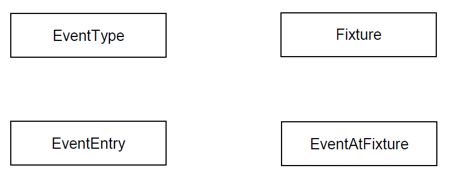
\includegraphics[width=0.5\paperwidth]{C:/Users/Admin/Desktop/Github/question_bank/LyX/static/img/9569-NYJC-2020-P1-Q5}
\par\end{center}
\begin{enumerate}
\item Copy and draw lines on \textbf{Figure 6} to show the degree of any
\textbf{three} relationships that exist between the four entities
shown. {[}3{]}
\item The following SQL statement is intended to make a table to represent
the Athlete relation. The statement contains some errors. 
\noindent \begin{center}
\textbf{Figure 7}
\par\end{center}

\noindent %
\noindent\begin{minipage}[t]{1\columnwidth}%
\texttt{CREATE TABLE Athlete ( }

\texttt{\qquad{}PRIMARY KEY AthleteID, }

\texttt{\qquad{}VARCHAR(50) Surname, }

\texttt{\qquad{}VARCHAR(30) Forename, }

\texttt{\qquad{}DATE DateOfBirth, }

\texttt{\qquad{}VARCHAR(6) Gender, }

\texttt{\qquad{}VARCHAR(30) TeamName }

\texttt{) }%
\end{minipage}

You may assume that all of the data types used in \textbf{Figure 7}
are valid and the field lengths are appropriate. State \textbf{two}
errors that have been made. \hfill{}{[}2{]}
\item State two reasons why database designs, such as this one, are usually
normalised. \hfill{}{[}2{]}
\item A list is to be produced of the names of all athletes who are competing
in the fixture that is taking place on 17/09/20. The list must include
the \texttt{Surname}, \texttt{Forename} and \texttt{DateOfBirth} of
these athletes and no other details. The list should be presented
in alphabetical order by Surname. With reference to the database design
shown in Figure 3, write an SQL query to produce the list. \hfill{}{[}5{]}
\item An IT consultant is suggesting changing to the use of a NoSQL database
instead.
\begin{enumerate}
\item Describe two advantages that a NoSQL database have over a SQL database.
\hfill{} {[}4{]}
\item Explain with reasons if you agree or disagree with making the change.
\hfill{}{[}2{]}
\end{enumerate}
\end{enumerate}
{[}SPLIT\_HERE{]}
\item \textbf{{[}NYJC/PRELIM/9569/2020/P1/Q6{]} }

Computers connected to the Internet use the TCP/IP suite of protocols
for data transmission.
\begin{enumerate}
\item What is a protocol? {[}1{]}
\item The TCP/IP stack is divided into four layers. One of these is the
application layer protocol. \textbf{Table 1} shows four different
scenarios that all use the TCP/IP protocol. Complete \textbf{Table
1} by writing the name of the particular \textbf{application layer
protocol} that would be used to transfer data during each operation.
You must give a different answer in each case.
\noindent \begin{center}
\textbf{Table 2}
\par\end{center}

\noindent \begin{center}
\begin{tabular}{|c|l|c|}
\hline 
 & \textbf{Operation} & \textbf{Application Layer Protocol }\tabularnewline
\hline 
\hline 
\textbf{(i)} & Managing a server remotely  & \tabularnewline
\hline 
\textbf{(ii)} & Retrieving e-mail from an e-mail server & \tabularnewline
\hline 
\textbf{(iii)} & Viewing a sports news web page using a web browser  & \tabularnewline
\hline 
\textbf{(iv)} & Accessing your online bank account using a web browser & \tabularnewline
\hline 
\end{tabular}
\par\end{center}

{[}4{]}
\item A student uses the following URL to download a copy of a previous
year\textquoteright s Computing exam paper.

$\mathtt{\underset{A}{\underbrace{https}}://\underset{B}{\underbrace{www.nanyang.moe.sg}}\underset{C}{\underbrace{/gce/computing/2019H2Computing2.pdf}}}$
\begin{enumerate}
\item Describe the \textbf{three} labelled parts (\texttt{A}, \texttt{B}
and \texttt{C}) of this URL.. \hfill{} {[}3{]}
\item State the top-level domain part in the URL. \hfill{} {[}1{]}
\end{enumerate}
\item To access the exam paper, the student\textquoteright s computer might
need to make use of a Domain Name System (DNS) query which is transmitted
to a DNS server.
\begin{enumerate}
\item What is the role of a DNS server? . \hfill{}{[}2{]}
\item In some circumstances the student\textquoteright s computer will not
need to contact a remote DNS server to access a resource. Describe
\texttt{two} situations when a DNS query will \texttt{not} be sent
to a remote DNS server. . \hfill{}{[}2{]}
\end{enumerate}
\item In the process of requesting a web page, a browser will generate an
HTTP GET request.
\begin{enumerate}
\item In which layer of the TCP/IP stack is the browser operating? . \hfill{}{[}1{]}
\item Explain why the student\textquoteright s computer might need to make
several HTTP GET requests to display one web page. . \hfill{}{[}2{]}
\item The HTTP GET requests are being sent to port 80 on the remote machine.
The browser has been allocated a \textbf{client port number}. What
is meant by a client port number?. \hfill{} {[}1{]}
\end{enumerate}
\end{enumerate}
{[}SPLIT\_HERE{]}
\item \textbf{{[}NYJC/PRELIM/9569/2020/P1/Q7{]} }

Below is a numbered list of the names of some of the legislation that
applies in situations where computers are used:

1. Copyright, Designs and Patents Act 

2. Computer Misuse Act 

3. Regulation of Investigatory Powers Act 

4. Health and Safety Regulations 5. Data Protection Act

For each of the situations given below, identify the relevant legislation
which is being followed. Write the number that corresponds to the
appropriate legislation in each situation.
\begin{enumerate}
\item {}
\begin{enumerate}
\item Marcus wanted an MP3 of a recent song so he went to an online music
store. After paying he was able to immediately download the purchased
song. \hfill{}{[}1{]}
\item A new workstation is installed in an office and an assessment is performed
regarding the lighting for the workstation and the positioning of
the desk, monitor and chair. \hfill{}{[}1{]}
\item Mr Smith hands over his 50-character encryption key in response to
a request from the authorities investigating a fraud case. \hfill{}{[}1{]}
\end{enumerate}
\item The operators of a number of multi-storey car parks have installed
systems to scan and recognise number plates. The system is used at
both the entrance and exit of the car parks so that the arrival and
leaving times can be recorded.

Customers can set up an account so that money is automatically debited
when their car number plate is recognised as the car leaves the car
park. Customers who do not have an account can use their mobile phones
to pay the car parking fees by sending a text message to a specified
number with their number plate details and length of stay.

As these car parks are based around Singapore, the company also collects
location specific data. 
\begin{enumerate}
\item The company will need to follow the Data Protection Act as they will
be storing personal data. What is meant by personal data? \hfill{}{[}1{]}
\item Why might the storing of number plate details, mobile phone numbers
and location specific data be a concern for privacy campaigners? \hfill{}
{[}2{]}
\end{enumerate}
\item Explain with specific examples why a code of conduct for computing
professionals is necessary. \hfill{} {[}3{]}
\end{enumerate}
{[}SPLIT\_HERE{]}
\end{enumerate}
 
\end{document}
